\documentclass{sigchi-ext}
% Please be sure that you have the dependencies (i.e., additional
% LaTeX packages) to compile this example.
\usepackage[T1]{fontenc}
\usepackage{textcomp}
\usepackage[scaled=.92]{helvet} % for proper fonts
\usepackage{graphicx} % for EPS use the graphics package instead
\usepackage{balance}  % for useful for balancing the last columns
\usepackage{booktabs} % for pretty table rules
\usepackage{ccicons}  % for Creative Commons citation icons
\usepackage{ragged2e} % for tighter hyphenation

% Some optional stuff you might like/need.
% \usepackage{marginnote} 
% \usepackage[shortlabels]{enumitem}
% \usepackage{paralist}
% \usepackage[utf8]{inputenc} % for a UTF8 editor only

%% EXAMPLE BEGIN -- HOW TO OVERRIDE THE DEFAULT COPYRIGHT STRIP --
% \copyrightinfo{Permission to make digital or hard copies of all or
% part of this work for personal or classroom use is granted without
% fee provided that copies are not made or distributed for profit or
% commercial advantage and that copies bear this notice and the full
% citation on the first page. Copyrights for components of this work
% owned by others than ACM must be honored. Abstracting with credit is
% permitted. To copy otherwise, or republish, to post on servers or to
% redistribute to lists, requires prior specific permission and/or a
% fee. Request permissions from permissions@acm.org.\\
% {\emph{CHI'14}}, April 26--May 1, 2014, Toronto, Canada. \\
% Copyright \copyright~2014 ACM ISBN/14/04...\$15.00. \\
% DOI string from ACM form confirmation}
%% EXAMPLE END

\copyrightinfo{Permission to make digital or hard copies of all or part of this
  work for personal or classroom use is granted without fee provided that
  copies are not made or distributed for profit or commercial advantage and
  that copies bear this notice and the full citation on the first page.
  Copyrights for components of this work owned by others than ACM must be
  honored. Abstracting with credit is permitted. To copy otherwise, or
  republish, to post on servers or to redistribute to lists, requires prior
  specific permission and/or a fee. Request permissions from
  permissions@acm.org.}

% Paper metadata (use plain text, for PDF inclusion and later
% re-using, if desired).  Use \emtpyauthor when submitting for review
% so you remain anonymous.
\def\plaintitle{Ritchie the DeskBuddy: 3D Printed Robot Avatar for Event Reminding}
\def\plainauthor{}
\def\emptyauthor{}
\def\plainkeywords{Ambient Device; Tangible Interface; Personification; 3D Printed Robots}
\def\plaingeneralterms{Documentation, Standardization}

\title{Ritchie the DeskBuddy: 3D Printed Robot Avatar for Event Reminding}

\numberofauthors{2}
% Notice how author names are alternately typesetted to appear ordered
% in 2-column format; i.e., the first 4 autors on the first column and
% the other 4 auhors on the second column. Actually, it's up to you to
% strictly adhere to this author notation.
\author{%
  \alignauthor{%
    \textbf{Dhananjai Hariharan}\\
    \affaddr{Rochester Institute of\\Technology} \\
    \affaddr{Rochester, NY 14623, USA} \\
    \affaddr{dh1723@rit.edu} }\alignauthor{%
    \textbf{Tiago Justino}\\
    \affaddr{Rochester institute of\\Technology} \\
    \affaddr{Rochester, NY, 14623, USA}\\
    \email{tvj6825@rit.edu} } }

% Make sure hyperref comes last of your loaded packages, to give it a
% fighting chance of not being over-written, since its job is to
% redefine many LaTeX commands.
\definecolor{linkColor}{RGB}{6,125,233}
\hypersetup{%
  pdftitle={\plaintitle},
%  pdfauthor={\plainauthor},
  pdfauthor={\emptyauthor},
  pdfkeywords={\plainkeywords},
  bookmarksnumbered,
  pdfstartview={FitH},
  colorlinks,
  citecolor=black,
  filecolor=black,
  linkcolor=black,
  urlcolor=linkColor,
  breaklinks=true,
}

% \reversemarginpar%

\begin{document}

\maketitle

% Uncomment to disable hyphenation (not recommended)
% https://twitter.com/anjirokhan/status/546046683331973120
\RaggedRight{} 

% Do not change the page size or page settings.
\begin{abstract}
  Ritchie The DeskBuddy is a 3D printed robotic tiger that works as an ambient
  device for reminding and notifying users about events relevant to their life.
  In this project, we attempt a different approach to combine digital
  information into a physical object, personified by an avatar. Through the use
  of such an ambient device, we seek to be able to drive user reaction and to
  also form an emotional bond with the user. We also aim that such a device can
  be used to imbibe new habits in users.
\end{abstract}

\keywords{\plainkeywords}

\category{H.5.2}{Information interfaces and presentation}{User Interfaces}

\section{Introduction}

There are a wide variety of resources available to people to keep track of
events and activities, remind them about these, and to make them more
productive. Two approaches are commonly used: 1. using physical reminders such
as post-it notes and diaries. The drawback here is that the user is physically
constrained. For example if the user has post-it notes at home, these notes
aren't accessible when she is in the library; and 2. using software reminders,
such as Google Keep and Google Calendar. Although they are available to use for
free, these are easy to ignore as they only exist virtually (only provide
simple notifications) and are not reflected sufficiently enough in the physical
world.

This project attempts a new approach to this application. What if it were
possible for a physical object in a user's space that could draw attention and
spark user reaction in a more effective manner? What if there could be an
object that can play the role of a friend that reminds a person about the
occurrence of an event? Wouldn't it be great if someone were to tell you to
stop what you were doing and keep up with your new year resolution of running
5K everyday? Graphical User Interfaces, by their nature, do not create an
emotional bond with a user in most interfaces. Having an emotional bond with an
object can greatly enhance user experience with that particular object,
irrespective of the simplicity of its purpose.


Ritchie the DeskBuddy is just the device for the role. Ritchie is a 3D printed
robotic tiger that sits on a user's desk and reminds them of events or
activities that need to be done. As an internet-connected device, Ritchie can
be of great utility when provided with pertinent data sources. To be clear,
Ritchie is not an AI robot. It cannot tell you what you need to do, or tell you
about the weather. Nor can it specifically remind you to buy some eggs on your
way back home. What Ritchie can do is wave its arms and move around to get your
attention about something important. The rest is upto the user to check on the
topic of concern. The events can range anything from small everyday events to
more important things that demand immediate action.

\section{Related Work}

Peek et.\ al \cite{peek2009hangsters} describe \textit{Hangster}, an ambient
display that embodies virtual interactions using physical devices hanging on
strings. These devices are designed to look like personalized avatars.
\textit{Hangster} allows a person to see their friend's status (online/offline)
on a messaging application (by lowering/raising the avatar), and allow some
simple interactions - e.g.\ initiate a conversation by gently tugging on the
avatar string, show notifications by moving. \textit{Dino}\footnote{Dino -
Ambient Display Creature: https://www.youtube.com/watch?v=AvST9wjrkC4} is an
ambient display that controls a physical object to react to the nature of
conversations on a chat application. By studying the content of the
conversation, the `egg' moves to show whether it is happy, sad, angry or calm.
Similarly, \textit{Availabot}\footnote{Availabot:
https://www.youtube.com/watch?v=w0voYnEjFcQ} is a computer-controlled push
puppet that stands or falls down to reflect a friend's availability
(online/offline status) on a chat application.

Jafarinaimi et.\ al \cite{jafarinaimi2005breakaway} describe
\textit{Breakaway}, an ambient display that attempts to encourage people who
sit for long periods to take more frequent breaks. This is implemented using a
shape-changing artistic sculpture object. User's position and posture is
tracked using various sensors. Shape and movement of the device reflects the
user's pose - upright when the user takes a break, and slouching when the
person has been sitting for extended periods. Similar to \textit{Breakaway},
\textit{MoveLamp} \cite{fortmann2013make} keeps track of a person's physical
activity at the workplace and attempts to encourage physical activity when a
person has been sitting for long periods. This made use of a pedometer
application on a smartphone, in combination with software on a computer to
control an ambient lamp that changed color from green to red to make the user
aware that they need to move. Rogers et.\ al \cite{rogers2010ambient}
investigated whether ambient displays can be used to influence behavioral
changes among people. In this study, they installed twinkly lights in the
carpets to unconsciously guide people to take the stairs. A large ambient
display in the common area was used to visualize the number of people using the
stairs vs.\ those that chose to use the elevator. While each of these were
implemented differently, they shared a common goal of nudging a user towards an
action and observing common behavioral changes over extended periods of time.

In \textit{Tangible Bits} \cite{ishii1997tangible}, Hiroshi Ishii proposes the
concept of coupling the digital world (bits of information) into a physical
object, thereby making it `tangible'. In line with this concept, Ritchie The
DeskBuddy would be a Tangible Bit, where the object would mirror digital
information and events, acting as a `phicon', or a physical icon.
\textit{ReaDIYmate}\footnote{ReaDIYmate: http://readiymate.com/} is a
commercially available DIY (Do-It-Yourself) kit for building internet-connected
paper objects that react to events in the digital world.  Similarly, few other
devices exist that physically react to digital events and interactions -
\textit{Olly}\footnote{Olly: http://www.ollyfactory.com/} is a device that
releases a scent for certain digital events/interactions. Similarly,
\textit{Polly}\footnote{Polly project: http://www.ollyfactory.com/polly/} is a
device that releases a ball of candy for certain digital events/interactions.

\begin{marginfigure}[-35pc]
  \begin{minipage}{\marginparwidth}
    \centering
    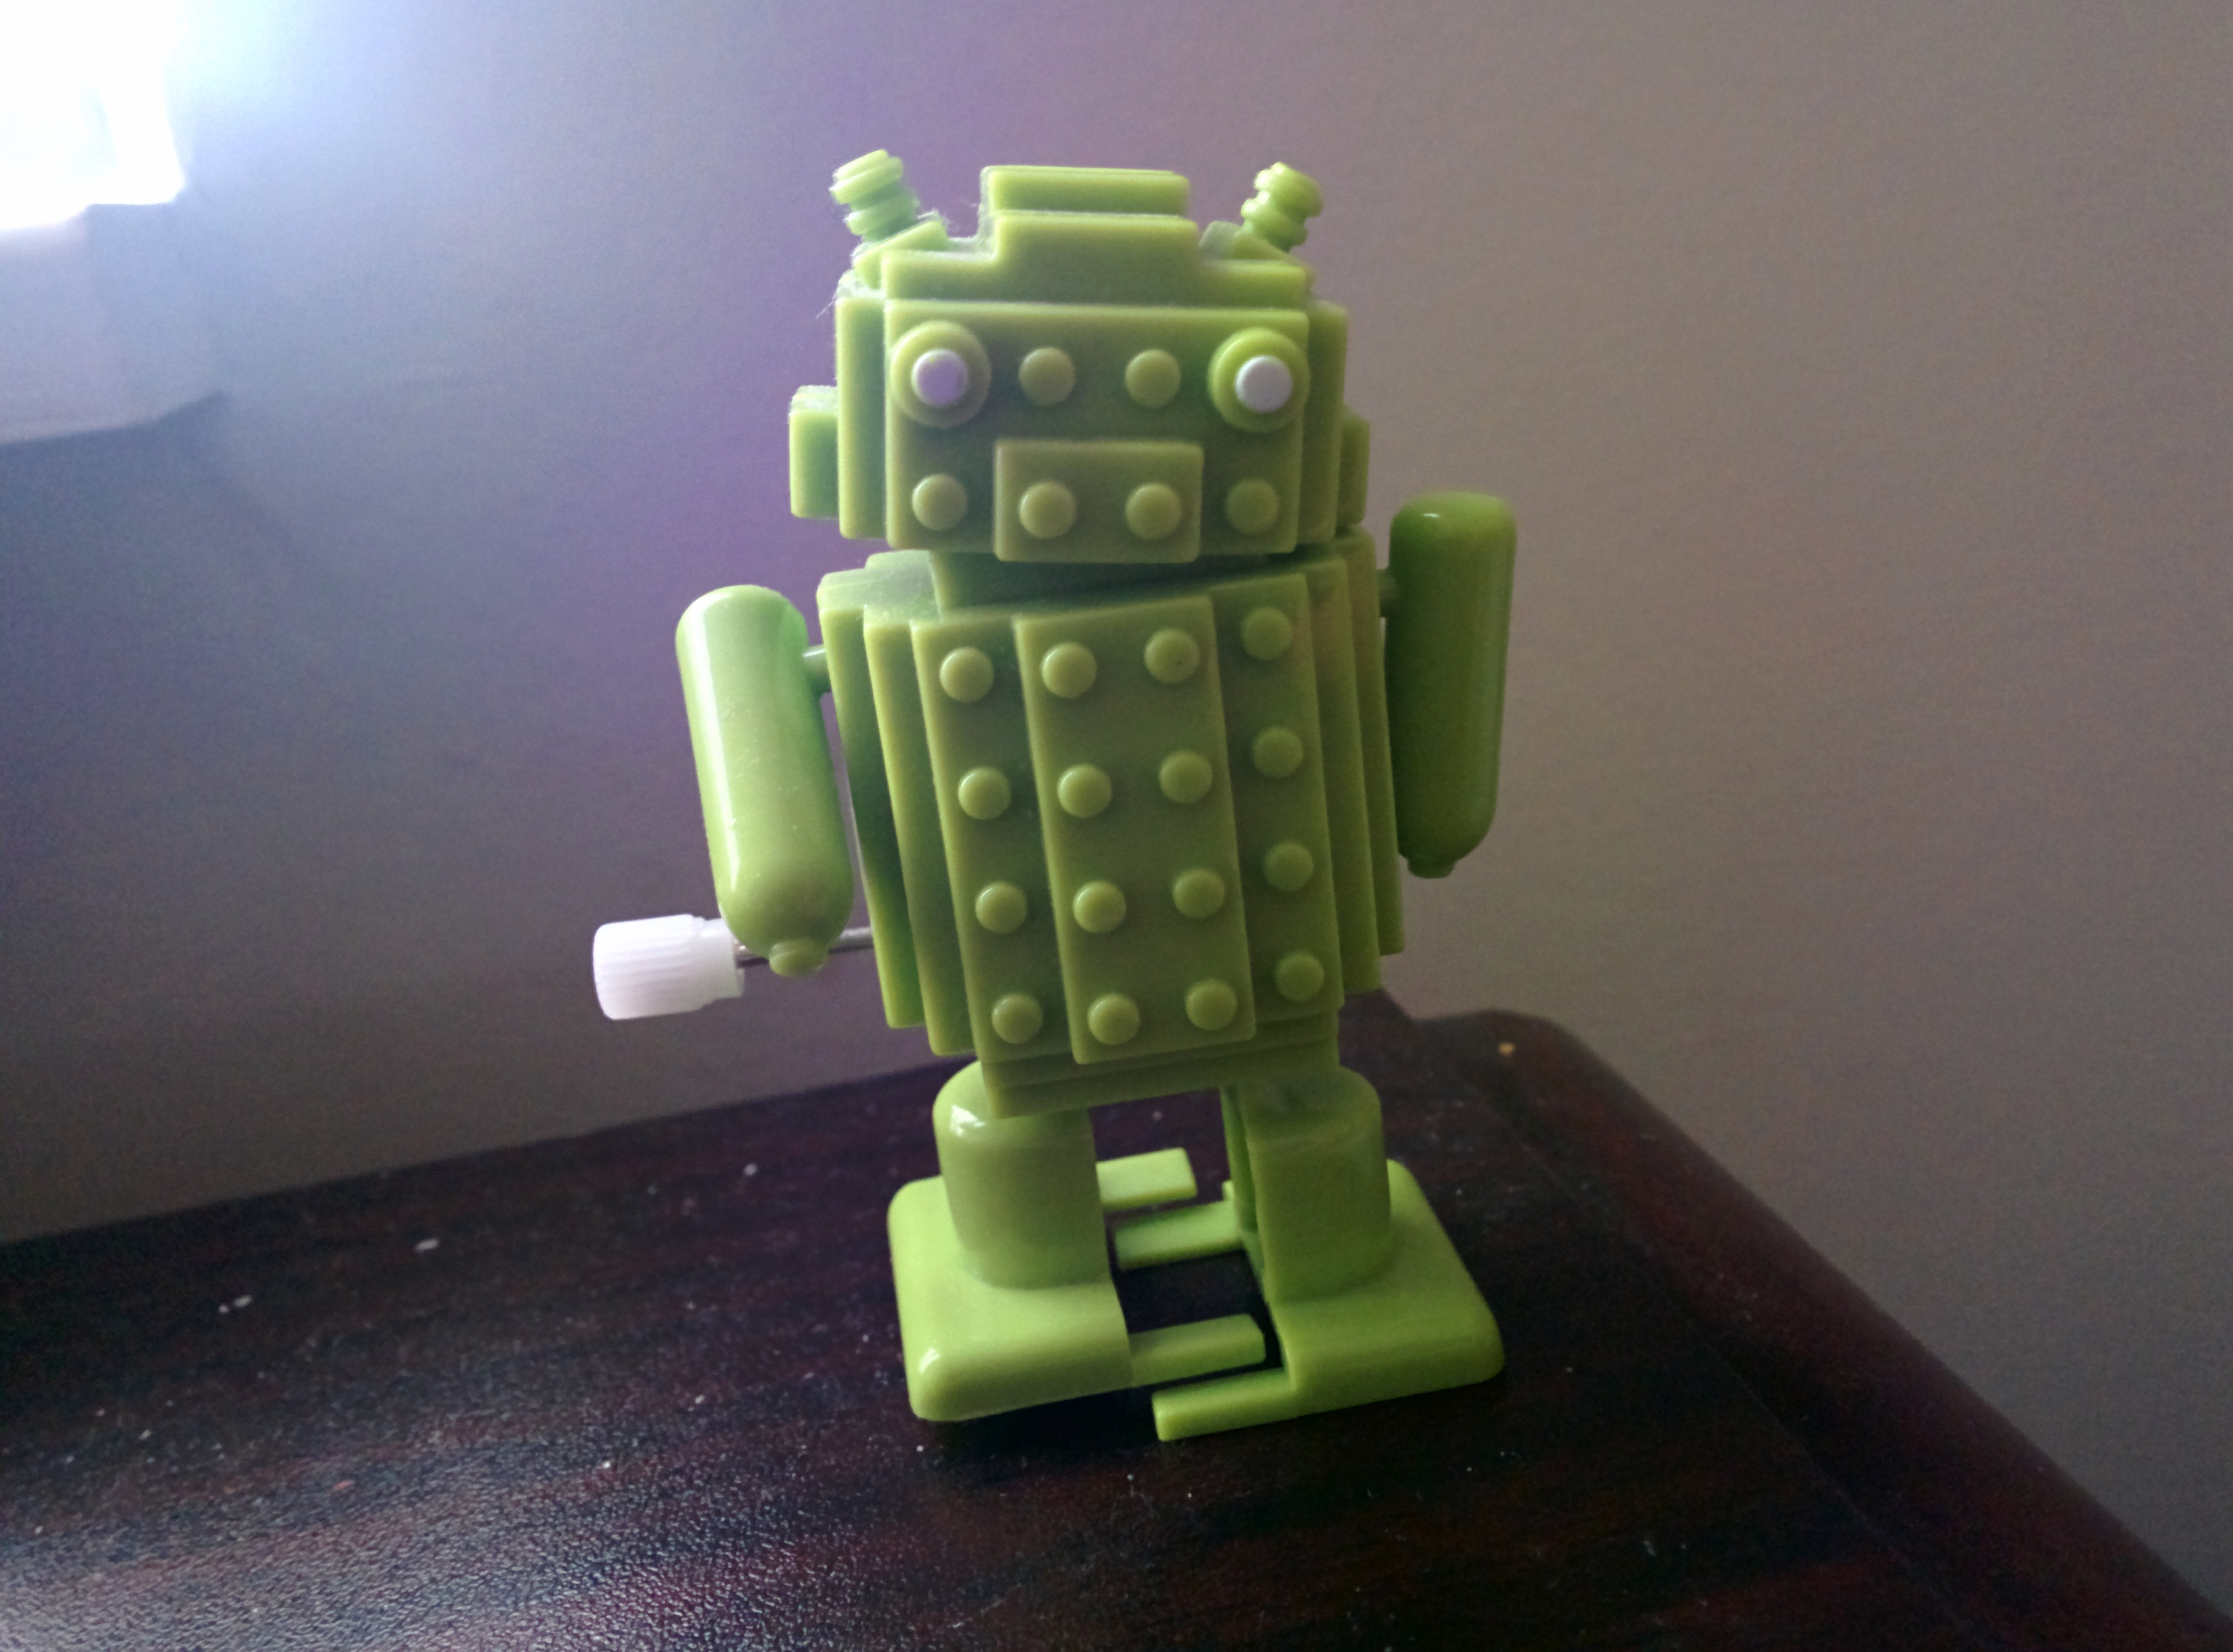
\includegraphics[width=0.9\marginparwidth]{../photos/android}
    \caption{Android toy that will be used to inspire Ritchie's design.}
    \label{fig:android}
  \end{minipage}
\end{marginfigure}

Besides the above mentioned research and projects, there is sufficient work in
the area of 3D printed robots and robot parts\cite{megaro2015interactive,
schulz2015interactive}\footnote{Instructables page: ``GearBot: A Dual-speed,
Gear-driven robot'':
http://www.instructables.com/id/GearBot-A-Dual-Speed-Gear-Driven-Bot/?ALLSTEPS}\footnote{Cubify
- Commercial 3D printed parts for custom designed robots:
http://cubify.com/store/mrn}, as well as numerous resources for accessing 3D
models of robots and parts for 3D printing.

\section{Project Description}

Ritchie The DeskBuddy is a 3D printed robotic tiger that sits on a user's desk
and reminds them of events or activities that need to be done.
Figure~\ref{fig:android} shows an Android toy that will be used as reference
for
Ritchie's design.

\subsection{Information Displayed}

The device would reflect reminders, events and tasks relevant to a user. The
same concept can be used to developing and practicing some new habits as well,
e.g.\ reading one chapter of a book everyday, running 5K, practice sketching
etc.

\subsection{Data Source}

For this project, Google Calendar\footnote{Google Calendar API:
https://developers.google.com/google-apps/calendar/} will be used as the data
source, as it is already widely used by many users as an application for
recording activities and keeping track of events.

\subsection{Device abilities}

The 3D printed robot will be able to do the following:
\begin{itemize}
  \item Perform a waving action (arm movement);
  \item Move on a flat surface (walk/drive);
  \item Play certain sounds for certain events;
  \item Blink lights to attract attention.
\end{itemize}

\subsection{Mapping of information to visualization}

The robot will be made to wave its arms when a \textbf{regular event} occurs. A
user can acknowledge this by simply tapping it. For events that occur over long
periods of time, the robot will repeat this behavior as a gentle reminder,
after a certain time period. When an \textbf{important event} is about to
occur, the robot will wave its arms and run around in a circle, while making
some sounds so as to draw attention. Events flagged as \textbf{tasks} or
\textbf{habits}, will be shown through similar device behavior. A user can
register task completion by lifting and shaking the robot, before placing it
back. The robot will respond by playing a sound to acknowledge this. For each
of these event scenarios, different light patterns will also be used to enhance
the visual effect.

\subsection{Components}

The following components will be used to build Ritchie the DeskBuddy:

\begin{itemize}
  \item Particle Photon;
  \item 1200mAh Lithium battery;
  \item Photon battery shield;
  \item Continuous Rotation Micro Servo (x1);
  \item 180deg rotation Micro Servo (x1);
  \item Accelerometer;
  \item Piezoelectric speaker;
  \item LEDs.
\end{itemize}

\subsection{Implementation Steps}

The following steps will be taken for the development of this project:

\begin{itemize}
  \item Study Google Calendar API:
  \begin{itemize}
    \item Authenticate to google calendar;
    \item Get list of events from google calendar;
  \end{itemize}
  \item Access google calendar API from Photon;
  \item Prototype robot abilities (breadboard):
  \begin{itemize}
    \item Use continuous motor with photon;
  \end{itemize}
  \item Prototype robot movement with continuous motor;
  \item Prototype arms movement with servo motor;
  \item Design and 3D print robot case;
  \item Assemble robot;
  \item Prepare demo;
  \item Record and edit video;
  \item Write final report.
\end{itemize}


%\marginpar{%
%  \vspace{-45pt} \fbox{%
%    \begin{minipage}{0.925\marginparwidth}
%      \textbf{Good Utilization of the Side Bar} \\
%      \vspace{1pc} \textbf{Preparation:} Do not change the margin
%      dimensions and do not flow the margin text to the
%      next page. \\
%      \vspace{1pc} \textbf{Materials:} The margin box must not intrude
%      or overflow into the header or the footer, or the gutter space
%      between the margin paragraph and the main left column. The text
%      in this text box should remain the same size as the body
%      text. Use the \texttt{{\textbackslash}vspace{}} command to set
%      the margin
%      note's position. \\
%      \vspace{1pc} \textbf{Images \& Figures:} Practically anything
%      can be put in the margin if it fits. Use the
%      \texttt{{\textbackslash}marginparwidth} constant to set the
%      width of the figure, table, minipage, or whatever you are trying
%      to fit in this skinny space.
%    \end{minipage}}\label{sec:sidebar} }

%\begin{figure}
%  \includegraphics[width=0.9\columnwidth]{figures/sigchi-logo}
%  \caption{Insert a caption below each figure.}~\label{fig:sample}
%\end{figure}

% \begin{figure}
%   \includegraphics[width=.9\columnwidth]{figures/ea-figure2}
%   \caption{If your figure has a light background, you can set its
%     outline to light gray, like this, to make a box around
%     it.}\label{fig:bats}
% \end{figure}

%\begin{marginfigure}[-35pc]
%  \begin{minipage}{\marginparwidth}
%    \centering
%    %\includegraphics[width=0.9\marginparwidth]{figures/cats}
%    \caption{In this image, the cats are tessellated within a square
%      frame. Images should also have captions and be within the
%      boundaries of the sidebar on page~\pageref{sec:sidebar}. Photo:
%      \cczero~jofish on Flickr.}~\label{fig:marginfig}
%  \end{minipage}
%\end{marginfigure}

%\begin{figure*}
%  \centering
%  \includegraphics[width=1.4\columnwidth]{figures/map}
%  \caption{In this image, the map maximizes use of space. You can make
%    figures as wide as you need, up to a maximum of the full width of
%    both columns. Note that \LaTeX\ tends to render large figures on a
%    dedicated page. Image: \ccbynd~ayman on Flickr.}~\label{fig:cats}
%\end{figure*}

%\marginpar{\vspace{-23pc}So long as you don't type outside the right
%  margin or bleed into the gutter, it's okay to put annotations over
%  here on the left, too; this annotation is near Hawaii. You'll have
%  to manually align the margin paragraphs to your \LaTeX\ floats using
%  the \texttt{{\textbackslash}vspace{}} command.}

%\begin{margintable}[1pc]
%  \begin{minipage}{\marginparwidth}
%    \centering
%    \begin{tabular}{r r l}
%      & {\small \textbf{First}}
%      & {\small \textbf{Location}} \\
%      \toprule
%      Child & 22.5 & Melbourne \\
%      Adult & 22.0 & Bogot\'a \\
%      \midrule
%      Gene & 22.0 & Palo Alto \\
%      John & 34.5 & Minneapolis \\
%      \bottomrule
%    \end{tabular}
%    \caption{A simple narrow table in the left margin
%      space.}~\label{tab:table2}
%  \end{minipage}
%\end{margintable}

\balance{}

\bibliographystyle{SIGCHI-Reference-Format}
\bibliography{references}

\end{document}

%%% Local Variables:
%%% mode: latex
%%% TeX-master: t
%%% End:
